\chapter{Дифференциал тоололын үндсэн теоремүүд}
\section{Функцийн дифферинциал}

\begin{definition}
$y=f(x)$ функц $x=a$ агуулсан төгсгөлөг интервалд $(b;c)$ дээр тодорхойлогдсон байг. Хэрэв $y=f(x)$ функцийн утгийн өөрчлөлт $f(a+h)-f(a)$-г $$f(a+h)-f(a)=Lh+\alpha(a,h), \qquad \lim_{h\to0}\frac{\alpha(a,h)}{h}=0 ,\quad L-\text{ тогтмол тоо}$$ хэлбэрт бичигдэж байвал $f(x)$ функцийг $x=a$ цэг дээр дифферинциачлагдах функц гэх ба $Lh$-г $f(x)$ функцийн $x=a$ цэг дээрх дифферинциал гээд $$dy=Lh$$ гэж тэмдэглэнэ.
\end{definition}
\begin{remark}
   $f(a+h)-f(a)=Lh+\alpha(a,h), \qquad \lim_{h\to0}\frac{\alpha(a,h)}{h}=0 ,\quad L-\text{ тогтмол тоо}$ хэлбэртэй бичигдэнэ гэдэг нь  
\[
0=\lim_{h\to0}\frac{f(a+h)-f(a)-Lh}{h}=\lim_{h\to0}\frac{f(a+h)-f(a)}{h}-L
\] буюу $$\lim_{h\to0}\frac{f(a+h)-f(a)}{h}=L$$ байна гэсэнтэй ижил юм. Иймд дараах теорем үнэн байна.
\end{remark}
\begin{theorem}[Дифференциал ба уламжлал] \(y=f(x)\) нь \(x=a\) цэг дээр дифференциалчлагддаг байх $\Leftrightarrow$ бол \(y=f(x)\) нь \(x=a\) цэг дээр уламжлалтай байна. Мөн \[
dy = f'(a)\,dx
\]
  өөрөөр хэлбэл $L=f'(a)$ байна. 
\end{theorem}
\begin{remark}
  Дифференциалчлагдах гэдэг нь функцын утгийг тухайн цэгийн орчинд нь шугаман функцээр сольж болно гэсэн үг.
\[
f(a+h)=f(a)+f'(a)h+\alpha(a,h)\approx f(a)+f'(a)h.
\] Хэрэв $a+h=x$ гэж орлуулбал $f(a+h)=f(x)\approx f(a)+f'(a)h=f(a)+f'(a)(x-a)$
шүргэгч шулуун гарна. Хэрэв $y=f(x)=x$ гэвэл $df=d(x)=1\cdot h$ тул $h=dx$ гэж үзэж болно.
\end{remark}
\begin{example}
  \(f(x)=x^2\) функц бүх цэг дээрээ уламжлалтай учир \(x=a\) дээр
\[
f'(a)=2a\Rightarrow  dy = 2a\,h=2a \,dx
\] байна. 
Хэрэв \(x\)-ийг \(dx=h\)  жижиг хэмжээгээр өөрчилвөл \( \Delta y = f(a+h)-f(a)=2a h + h^2\) болно. Иймд дифференциал \(dy=2a h\) ба \( \Delta y \) —ийн ялгаа \(h^2\) нь $\alpha(a,h)$ болно. Хэрэв $h$ маш бага бол $\alpha(a,h)$ нь тодорхойлолт ёсоор бараг тэг болно.
\end{example} 
\begin{example}[Дифференциал ашиглан ойролцоо утга тооцоолох]
$\sqrt{9.1}$-ийг ойролцоогоор бодъё.

Функцийг $y=\sqrt{x}$ гэж авбал:
\[
y' = \frac{1}{2\sqrt{x}}
\]

$9.1$ ба $9$-н зөрүү бага тул $a=9$, $h=dx = 9.1-9 = 0.1$.

\[
dy = y'(9)\cdot dx
\]

\[
y'(9) = \frac{1}{2\sqrt{9}} = \frac{1}{6}
\qquad \Rightarrow \qquad
dy = \frac{1}{6}\cdot 0.1 = 0.0167
\]

Тэгэхээр:
\[
\sqrt{9.1} \approx \sqrt{9}+dy = 3 + 0.0167 = 3.0167
\]

Тооны машинаар бодвол
\[
\sqrt{9.1} \approx 3.01662
\]
Дифференциалын ойролцоо утга таарч байна.
\end{example}
\section{Локал ба глобал экстремум}
\begin{definition}[Локал экстремум]
$f$ функц $x=a$ цэгийн орчинд тодорхойлогдсон байг. Өрөөр хэлбэл $(a-\delta;a+\delta)$ завсарыг агуулсан муж дээр тодорхойлогдсон байг. Хэрэв $\forall x\in(a-\delta,a+\delta)$ хувьд 
\[
f(x)\le f(a)\;\;(\text{эсвэл } f(x)\ge f(a))
\] байхаар $\delta>0$ тоо олддог бол $f(a)$-г тус функцийн \textbf{локал максимум} ( \textbf{локал минимум} ) гэнэ. Эдгээрийг нийлүүлээд \textbf{локал экстремум} гэнэ.
\end{definition}

\begin{definition}[Глобал экстремум]
$f$ нь $X$ муж дээр тодорхойлогдсон байг. Хэрэв $\forall x\in X$ хувьд 
\[
f(x)\le f(a)\quad(\text{эсвэл } f(x)\ge f(a))
\]
бол $f(a)$-г  тус фунцийн \textbf{глобал максимум} эсвэл Хамгийн их утга, ( \textbf{глобал минимум} эсвэл Хамгийн бага утга) гэнэ.
\end{definition}

\begin{remark}
Глобал экстремум нь бүх мужид хамгийн их/бага утга; локал экстремум нь зөвхөн тухайн цэгийн \emph{орчимд} хамгийн их/бага утга юм.
\end{remark}
\begin{example}
Дараах зурагт дүрслэгдсэн функцийн хувьд $A$ цэг бол локал максимум, $B$ цэг бол локал минимум, $C$ цэг бол локал максимум ч биш, локал минимум ч биш байна. График цааш үргэлжилэхгүй энэ зураг дээрх шиг бол үзүүрийн цэгүүд глобал максимум ба глобал минимум болно. 
\begin{center}
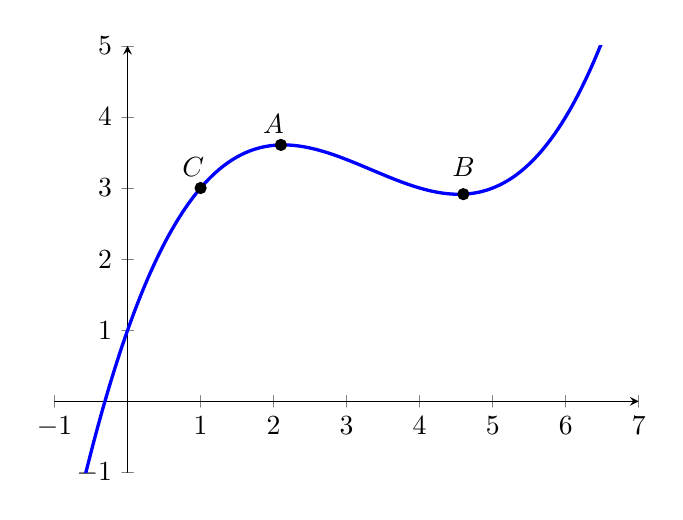
\begin{tikzpicture}[line cap=round,line join=round]
\begin{axis}[
  axis lines=middle,
  xmin=-1, xmax=7,
  ymin=-1, ymax=5,
  xtick={-1,0,...,7},
  ytick={-1,0,...,5},
  width=9cm, height=7cm
]
% Графикийг pgfplots-оор зурах (addplot):
\addplot[
  blue, very thick, samples=200, domain=-1:7, smooth
] { ((x)-1)*((x)-4)*((x)-5)/10 + 3 };

% Цэгүүдийг axis cs: ашиглан тавина
\addplot[only marks, mark=*] coordinates {(2.0998591391405212,3.6060967528584933)};
\node at (axis cs:2,3.9) {$A$};

\addplot[only marks, mark=*] coordinates {(4.598678018120027,2.9135372087404416)};
\node at (axis cs:4.6,3.3) {$B$};

\addplot[only marks, mark=*] coordinates {(1,3)};
\node at (axis cs:0.9,3.3) {$C$};

\end{axis}
\end{tikzpicture}
\end{center}
\end{example}

% ===============================================================
\section{Үндсэн теоремүүд}
\begin{theorem}[Ферма]
$f$ функц $x=a$ дээр \textbf{локал экстремум}-тай бөгөөд $f$ нь $a$ дээр дифференциалчлагддаг бол
\[
f'(a)=0
\] байна.
\end{theorem}

\begin{prof} 
$a$ цэг локал максимум тохиолдолд баталгаа хийе. Минимумын хувьд аналог. 

$f'(a)=\lim\limits_{x\to a} \dfrac{f(x)-f(a)}{x-a}$ байна. 
$x>a$ үед $\dfrac{f(x)-f(a)}{x-a}\le 0$, $x<a$ үед $\dfrac{f(x)-f(a)}{x-a}\ge 0$. Иймд $f'(a)=\lim\limits_{x\to a} \dfrac{f(x)-f(a)}{x-a}$  оршихийн тулд баруун зүүн хязгаарууд тэнцэх ёстой. Гэтэл баруун зүүн  хязгаарын утгууд тэнцүү бол зөвхөн $0$ байх боломжтой. Иймд $f'(a)=0$. 
\end{prof}
\begin{example}
$y=x^2-4x+3$ функцийн хувьд $A(2,-1)$ цэг бол локал минимум байна. $f'(x)=2x-4$ тул $f'(2)=0$ байна.
\begin{center}
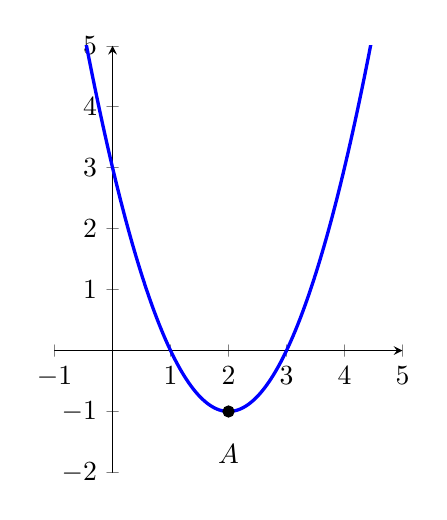
\begin{tikzpicture}[line cap=round,line join=round]
\begin{axis}[
  axis lines=middle,
  xmin=-1, xmax=5,
  ymin=-2, ymax=5,
  xtick={-1,0,...,5},
  ytick={-2,-1,...,5},
  width=6cm, height=7cm
]
% Графикийг pgfplots-оор зурах (addplot):
\addplot[
  blue, very thick, samples=200, domain=-1:5, smooth
] { ((x)-2)*((x)-2)-1 };

% Цэгүүдийг axis cs: ашиглан тавина
\addplot[only marks, mark=*] coordinates {(2,-1)};
\node at (axis cs:2,-1.7) {$A$};
\end{axis}
\end{tikzpicture}
\end{center}
$f(x)=x^3$ хувьд $f'(0)=0$ боловч $a=0$ цэг локал экстремум биш. Фермагийн теорем нь локал экстремум дээр уламжлалтай бол тэр нь $0$ байхыг батлаж байна. Харин уламжлал нь тэг байвал экстермум байх албагүй.
\begin{center}
\begin{tikzpicture}[scale=0.9]
\draw[->] (-2,0)--(2,0) node[right]{$x$};
\draw[->] (0,-2)--(0,2) node[above]{$y$};
\draw[domain=-1.3:1.3,smooth,variable=\x,blue,thick] plot({\x},{\x*\x*\x});
\fill (0,0) circle(2pt) node[above left]{$f'(0)=0$ (экстремум биш)};
\end{tikzpicture}
\end{center}

\end{example}
\begin{theorem}[Ролл]
$f$ нь $[a,b]$ дээр тасралтгүй, $(a,b)$ дээр дифференциалчлагддаг бөгөөд $f(a)=f(b)$ бол $\exists\,c\in(a,b)$: $f'(c)=0$.
\end{theorem}

\begin{prof}
$f$ нь $[a,b]$ дээр тасралтгүй учир $f$ хамгийн их/бага утгаа авна. Хэрэв $f$ тогтмол биш бол экстремум нь $(a,b)$ дотор цэгт оршино. Фермагийн теоремээр тэр экстермумийн цэг дээр $f'(c)=0$ болж батлагдав.
\end{prof}

\begin{center}
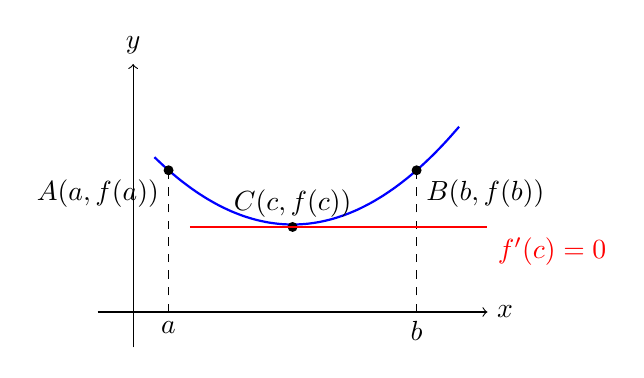
\begin{tikzpicture}[scale=0.9]
\draw[->] (-0.5,0)--(5,0) node[right]{$x$};
\draw[->] (0,-0.5)--(0,3.5) node[above]{$y$};
\draw[domain=0.3:4.6,smooth,variable=\x,blue,thick] plot({\x},{0.25*(\x-0.5)*(\x-4)+2});
\coordinate (A) at (0.5,2);
\coordinate (B) at (4,2);
\coordinate (C) at (2.25,1.2);
\fill (A) circle (2pt) node[below left]{$A(a,f(a))$};
\fill (B) circle (2pt) node[below right]{$B(b,f(b))$};
\fill (C) circle (2pt) node[above]{$C(c,f(c))$};
\draw[dashed] (0.5,0)--(0.5,2);
\draw[dashed] (4,0)--(4,2);
\draw[red,thick] (0.8,1.2)--(5,1.2) node[below right]{$f'(c)=0$};
\node[below] at (0.5,0){$a$};
\node[below] at (4,0){$b$};
\end{tikzpicture}
\end{center}

\begin{example}
$f(x)=x^2-4x+3$ дээр $[1,3]$ үед $f(1)=f(3)=0$, $f'(x)=2x-4=0\Rightarrow c=2$.
\end{example}

\begin{theorem}[Лагранжийн дундаж утгын теорем]
$f$ нь $[a,b]$ дээр тасралтгүй, $(a,b)$ дээр дифференциалчлагддаг бол $\exists\,c\in(a,b)$:
\[
f'(c)=\frac{f(b)-f(a)}{\,b-a\,}.
\]
\end{theorem}

\begin{prof}
$g(x)=f(x)-\dfrac{f(b)-f(a)}{b-a}(x-a)$. Тэгвэл $g(a)=g(b)$ бөгөөд Роллыг хэрэглэвэл $g'(c)=0$, өөрөөр хэлбэл $f'(c)=\dfrac{f(b)-f(a)}{b-a}$.
\end{prof}

\begin{remark}
Геометр утга: ямар нэг $c$ цэг дээрх шүргэгчийн налалт нь $A(a,f(a))$ ба $B(b,f(b))$ цэгүүдийг холбосон хөвчийн налалттай тэнцүү.
\end{remark}
%$$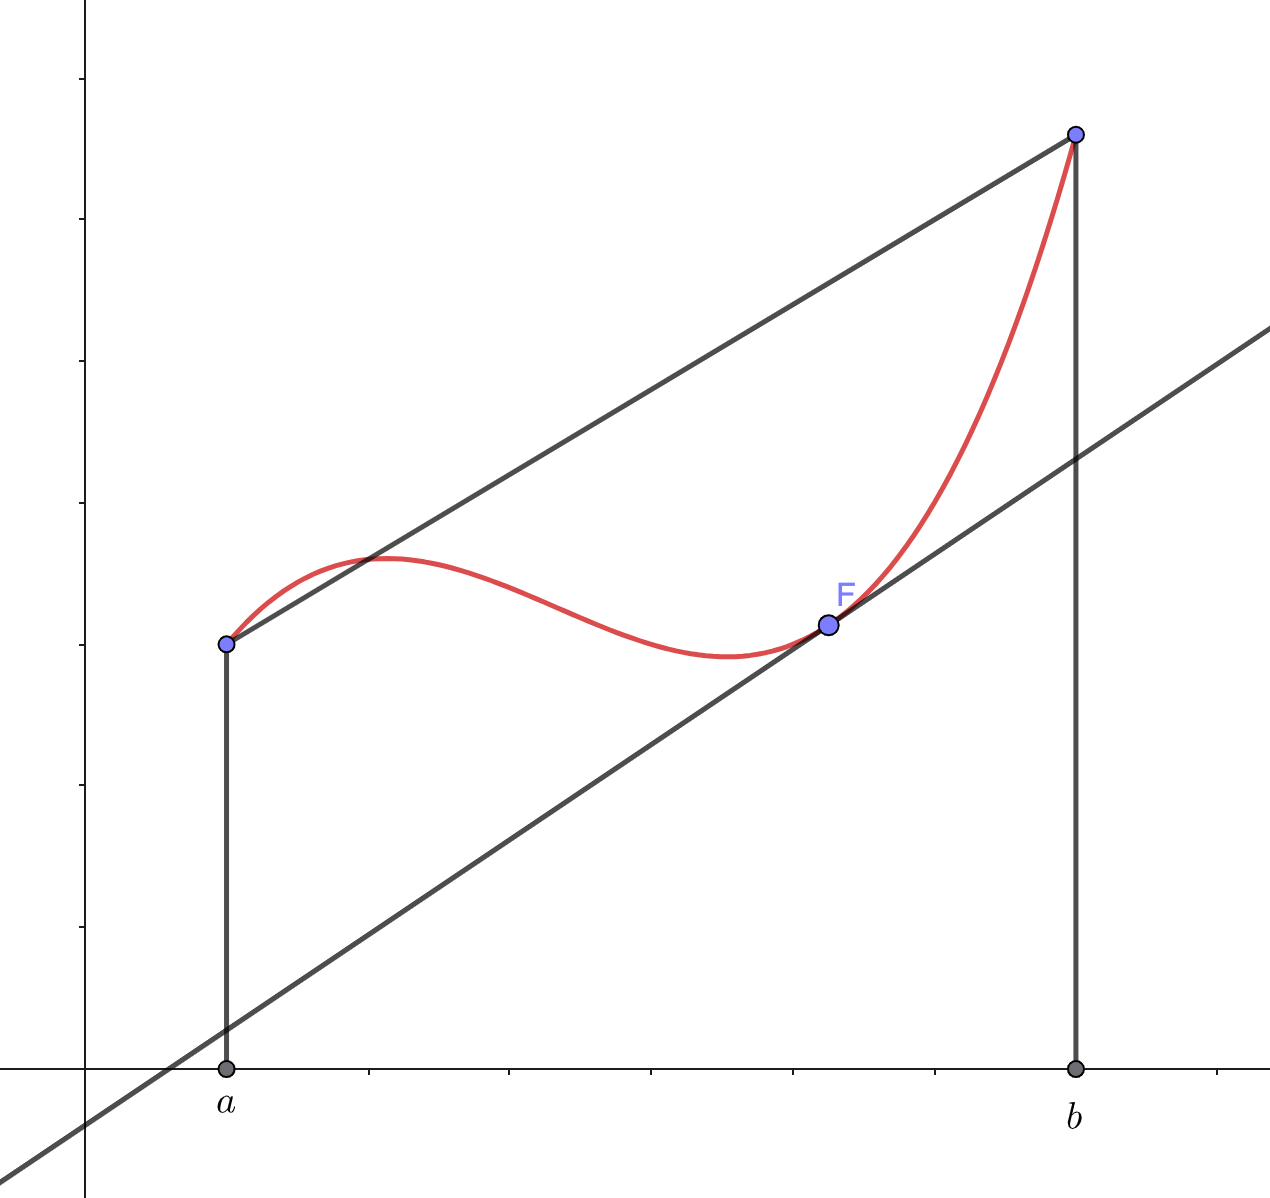
\includegraphics[scale=0.5]{pictures/IVT.png}$$
\begin{center}
\begin{tikzpicture}[scale=0.9]
\draw[->] (-0.5,2)--(8,2) node[right]{$x$};
\draw[->] (0,-0.5)--(0,7) node[above]{$y$};
\draw[domain=0:7.3,smooth,variable=\x,blue,thick] plot({\x},{0.1*(\x-1)*(\x-4)*(\x-5)+3});
\coordinate (A) at (1,3);
\coordinate (B) at (7,6.6);
\coordinate (C) at (5.25,3.13);
\fill (A) circle (2pt) node[left]{$A(a,f(a))$};
\fill (B) circle (2pt) node[right]{$B(b,f(b))$};
\fill (C) circle (2pt) node[below]{$C(c,f(c))$};
\draw[very thick,orange] (A)--(B) node[midway,left]{хөвчийн налалт $=\dfrac{f(b)-f(a)}{b-a}$};
\draw[very thick,red] (0,-0.4)--(8,4.96) node[right]{шүргэгчийн налалт $=f'(c)$};
\node[below] at (2.3,0){$c$};
\end{tikzpicture}
\end{center}

\paragraph{Жишээ.} 
\begin{enumerate}[itemsep=2pt]
\item $f(x)=x^2$ $[1,3]$: $\dfrac{9-1}{2}=4$, $f'(x)=2x\Rightarrow c=2$.
\item $f(x)=\sin x$ $[0,\pi]$: $\dfrac{0-0}{\pi}=0$, $f'(x)=\cos x\Rightarrow c=\dfrac{\pi}{2}$.
\item $f(x)=\ln x$ $[1,e]$: $\dfrac{1-0}{e-1}$, $f'(x)=1/x\Rightarrow c=e-1$.
\item $f(x)=x^3$ $[-1,1]$: $\dfrac{1-(-1)}{2}=1$, $f'(x)=3x^2\Rightarrow c=\pm 1/\sqrt{3}$.
\end{enumerate}
\begin{theorem}[Кошийн дундаж утгын теорем]
$f,g$ нь $[a,b]$ дээр тасралтгүй, $(a,b)$ дээр дифференциалчлагддаг бол $\exists\,c\in(a,b)$:
\[
\frac{f'(c)}{g'(c)}=\frac{f(b)-f(a)}{g(b)-g(a)}.
\]
\end{theorem}

\begin{prof}
$F(x)=f(x)-\lambda g(x)$, энд $\lambda=\dfrac{f(b)-f(a)}{g(b)-g(a)}$. Тэгвэл $F(a)=F(b)$, Роллоор $F'(c)=0\Rightarrow f'(c)=\lambda g'(c)$.
\end{prof}

\paragraph{Жишээ.}
\begin{enumerate}[itemsep=2pt]
\item $f(x)=\ln x,\ g(x)=x$ $[1,e]$: $\dfrac{f'(c)}{g'(c)}=\dfrac{1/c}{1}=\dfrac{1}{e-1}\Rightarrow c=e-1$.
\item $f(x)=\tan x,\ g(x)=x$ $[0,\pi/4]$: $\sec^2 c=\dfrac{1-0}{\pi/4}=\dfrac{4}{\pi}$.
\end{enumerate}

% ===============================================================
\section{Уламжлалын хэрэглээ}
\subsection{[Шүргэгч шулуун ба Нормал шулуун}
\begin{definition}[Шүргэгч шулуун]
$y=f(x)$ функц нь $x=a$ цэг дээр дифференциалчлагддаг гэж үзье.  
Дараах тэгшитгэлтэй:
\[
\boxed{y - f(a) = f'(a)\,(x - a).}
\] шулууныг $y=f(x)$ функц нь $x=a$ цэг дээрх шүргэгч шулуун гэнэ.
Энд $f'(a)$ нь шүргэгчийн налалт буюу тухайн цэг дэх муруйн чиг хандлагыг илэрхийлнэ.
\end{definition}
\begin{definition}[Нормал шулуун]
Муруйн $x=a$ цэгийг дайрсан, энэ цэг дээрх  шүргэгч шулуунд перпендикуляр шулууныг $x=a$ цэг дээрх \emph{нормал шулуун} гэнэ.  
Хэрэв $f'(a)\ne 0$ бол нормал шулууны налалт $m_\perp=-\dfrac{1}{f'(a)}$ бөгөөд тэгшитгэл нь:
\[
\boxed{y - f(a) = -\frac{1}{f'(a)}(x - a).}
\]
Хэрэв $f'(a)=0$ бол шүргэгч нь хэвтээ, нормал нь босоо шулуун $x=a$ байна.
\end{definition}

\begin{example}[Шүргэгч ба нормал: параметр функц]
 $x=\cos t,\; y=\sin t$ муруй нь тойргийг дүрсэлнэ. $t=\dfrac{\pi}{4}$ цэг дээр:
\[
\frac{dx}{dt}=-\sin t,\qquad \frac{dy}{dt}=\cos t
\quad\Rightarrow\quad
\frac{dy}{dx}=\frac{dy/dt}{dx/dt}=\frac{\cos t}{-\sin t}=-\cot t.
\]
$t=\dfrac{\pi}{4}$ үед \;$m_{\text{tan}}=\dfrac{dy}{dx}=-1$. Цэг нь
\[
P\Bigl(\tfrac{\sqrt2}{2},\,\tfrac{\sqrt2}{2}\Bigr).
\]
Иймд шүргэгчийн шулуун:
\[
\boxed{\,y-\tfrac{\sqrt2}{2}=-1\Bigl(x-\tfrac{\sqrt2}{2}\Bigr)\,}.
\]
Нормал нь шүргэгчид перпендикуляр тул \;$m_{\text{nor}}=1$:
\[
\boxed{\,y-\tfrac{\sqrt2}{2}=1\Bigl(x-\tfrac{\sqrt2}{2}\Bigr)\,}.
\]

\medskip
\begin{center}
\begin{tikzpicture}[scale=2,>=stealth]
  % Тэнхлэг
  \draw[->] (-1.4,0)--(1.4,0) node[right] {$x$};
  \draw[->] (0,-1.4)--(0,1.4) node[above] {$y$};

  % Тойрог x^2 + y^2 = 1
  \draw[thick] (0,0) circle (1);

  % Цэг P
  \coordinate (P) at ({sqrt(2)/2},{sqrt(2)/2});
  \fill (P) circle (1.2pt) node[above right] {$P\left(\tfrac{\sqrt2}{2},\tfrac{\sqrt2}{2}\right)$};

  % Шүргэгч: y - y0 = -1(x - x0)
  % Туслах хоёр цэг авч дүрслэх
  \draw[very thick,blue]
    (-1,2.3) -- (2,-0.5);

  % Нормал: y - y0 = 1(x - x0)
  \draw[very thick,red] (-1,-1) -- (1.5,1.5);

  % Нэгж тэмдэглэгээ
  \draw (1,0) node[below] {\small $1$};
  \draw (0,1) node[left] {\small $1$};
\end{tikzpicture}
\end{center}
\end{example}

% --- Нормал ба шүргэгч (далд өгөлт) ---
\begin{example}[Шүргэгч ба нормал: далд функц]
$F(x,y)=x^2+y^2-1=0$ тойрог дээр $\displaystyle y'=-\frac{F_x}{F_y}=-\frac{2x}{2y}=-\frac{x}{y}$.
\begin{itemize}
  \item $(0,1)$ дээр $y'=-\dfrac{0}{1}=0$ тул \emph{шүргэгч} хэвтээ: \;\; $\boxed{y=1}$.
  \item Харин \emph{нормал} нь перпендикуляр тул босоо: \;\; $\boxed{x=0}$.
\end{itemize}

\medskip
\begin{center}
\begin{tikzpicture}[scale=2,>=stealth]
  % Тэнхлэг
  \draw[->] (-1.4,0)--(1.4,0) node[right] {$x$};
  \draw[->] (0,-1.4)--(0,1.4) node[above] {$y$};

  % Тойрог
  \draw[thick] (0,0) circle (1);

  % Цэг Q = (0,1)
  \coordinate (Q) at (0,1);
  \fill (Q) circle (1.2pt) node[above left] {$Q(0,1)$};

  % Шүргэгч y=1
  \draw[very thick,blue] (-1.2,1)--(1.2,1) node[right] {\small шүргэгч $\,y=1$};

  % Нормал x=0
  \draw[very thick,red] (0,-1.2)--(0,1.2) node[above] {\small нормал $\,x=0$};

  % Нэгж тэмдэглэгээ
  \draw (1,0) node[below] {\small $1$};
  \draw (0,1) node[left] {\small $1$};
\end{tikzpicture}
\end{center}
\end{example}
\subsubsection{Өсөлт, бууралтын шинжилгээ}
\begin{definition}[Өсөх ба буурах функц]
$f$ функц $(a,b)$ завсарт тодорхойлогдсон байг. 
\begin{itemize}
  \item Хэрэв дурын $x_1,x_2\in(a,b)$ үед $x_1<x_2\Rightarrow f(x_1)<f(x_2)$ байвал $f$-ийг $(a,b)$ дээр \textbf{өсөх}  функц гэнэ.
  \item Хэрэв $x_1<x_2\Rightarrow f(x_1)>f(x_2)$ байвал $f$-ийг $(a,b)$ дээр \textbf{буурах} функц гэнэ.
\end{itemize}
\end{definition}

\begin{theorem}[Өсөлт–бууралтын тест]
$f$ функц $(a,b)$ дээр дифференциалчлагддаг ба бүх $x\in (a,b)$ хувьд \\
\begin{itemize}
    \item $f'(x) > 0, \text{бол } f \text{ өсөх функц},$
    \item $f'(x) < 0,  \text{бол } f \text{ буурах функц},$
    \item $f'(x) = 0, \text{бол } f \text{ тогтмол функц}$
\end{itemize}
 байна.
\end{theorem}
\begin{prof}
$\,f$ дифференциалчлагддаг, $x_1,x_2\in(a,b)$, $x_1<x_2$ байг. Лагранжийн дундаж утгын теоремыг санавал
\[
\exists\,c\in(x_1,x_2)\quad,\quad f'(c)=\frac{f(x_2)-f(x_1)}{x_2-x_1}.
\]
Хэрэв $\forall x\in (a,b)$ хувьд $f'(x)>0$ байвал $f'(c)>0$ тул $f(x_2)-f(x_1)>0$, өөрөөр хэлбэл $f(x_2)>f(x_1)$ буюу $f$ өсөх функц болно. Үүнтэй адил $f'(x)<0$ бол $f(x_2)<f(x_1)$ буюу $f$ буурах функц байна.
\end{prof}
\begin{example}
$f(x)=x^3-3x$.
\[
f'(x)=3x^2-3=3(x-1)(x+1).
\]
\begin{itemize}
  \item $f'(x)>0$ үед, өөрөөр хэлбэл $x<-1$ үед функц өснө. Мөн  $x>1$ үед функц өснө.
  \item $-1<x<1$ үед $f'(x)<0$ тул $f$ функц $-1<x<1$ үед буурна.
\end{itemize}
\begin{center}
    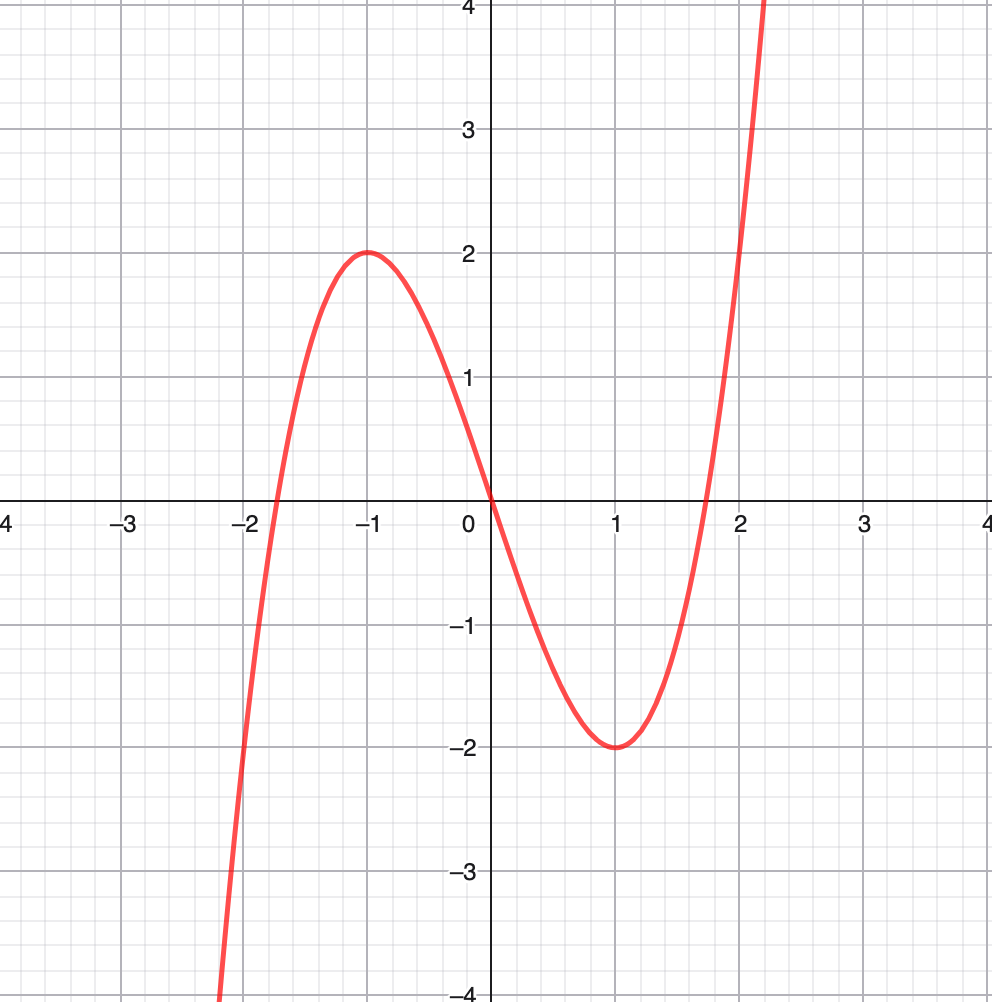
\includegraphics[scale=0.5]{pictures/x^3-3x.png}
\end{center}
\end{example}
 $f'(x)$-ийн тэмдэгийг мэдснээр функцийн өсөлт–бууралтыг мэдэх төдийгүй улмаар локал болон глобал экстремумын байршлыг тодорхойлдог. 

 Фермагийн теорем экстремум байхгүй цэгүүдйиг зааж өгдөг теорем юм. Өөрөөр хэлбэл $f'(a)\neq 0$ бол $x=a$ цэг экстремум биш юм. Харин $f'(a)= 0$ эсвэл $f'(a)$ оршин байхгүй бол $x=a$ цэг экстремум байж магадгүй.
 \begin{definition}
     Хэрэв $y=f(x)$ функцийн хувьд $f'(a)= 0$ эсвэл $f'(a)$ оршин байхгүй бол $x=a$ цэгийг $y=f(x)$ функцийн локал эксттермум байж магадгүй \textit{сэжигтэй цэг} гэнэ.
 \end{definition}
\begin{example}
$f(x)=x e^{-x}$ бол
\[
f'(x)=e^{-x}(1-x) 
\] байна.
$e^{-x}>0$ тул $f'(x)$-ийн тэмдэгийг $1-x$ тодорхойлно:
\[
\begin{cases}
f'(x)>0, & x<1 \;\Rightarrow\; f \text{ өсөх},\\
f'(x)<0, & x>1 \;\Rightarrow\; f \text{ буурах}.
\end{cases}
\]
$f'(x)=e^{-x}(1-x)=0\Rightarrow x=1 $ тул сэжигтэй цэг нь $x=1$ болно. График харвал 
\begin{center}
    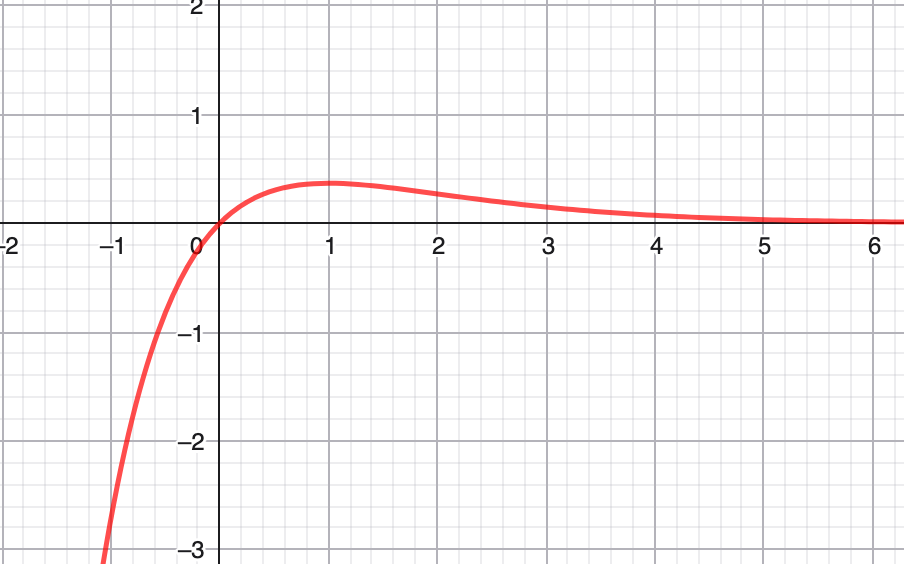
\includegraphics[scale=0.4]{pictures/xe^-x.png}
\end{center} 
$x=1$ цэг нь локал максимум ба 
$f(1)=e^{-1}$ нь \textbf{локал максимум утга} байна.
\end{example}
Дээрх жишээнээс дараах дүгнэлт хийж болно. 
\begin{theorem}
    $x=a$ цэг нь $y=f(x)$ функцийн сэжигтэй цэг байг. Хэрэв функц $(a-\delta;a)$ завсарт өсөөд (буураад), $(a;a+\delta)$ завсарт буурдаг (өсдөг) байх $\delta>0$ тоо олддог бол $x=a$ цэг $y=f(x)$ функцийн локал максимум (минимум)-н  цэг байна.
\end{theorem}

\begin{example}
$f(x)=x^2 e^{-x}$.
\[
f'(x)=e^{-x}(2x-x^2)=e^{-x}x(2-x).
\]
$f'(x)$-ийн тэмдэг:
\begin{itemize}
  \item $x<0$: $f'(x)<0$ (буурах),
  \item $0<x<2$: $f'(x)>0$ (өсөх),
  \item $x>2$: $f'(x)<0$ (буурах).
\end{itemize}
Тиймээс $x=0$ дээр \textbf{локал минимум}, $x=2$ дээр \textbf{локал максимум}.
\[
f(0)=0,\qquad f(2)=4e^{-2}.
\]
\end{example}
\begin{center}
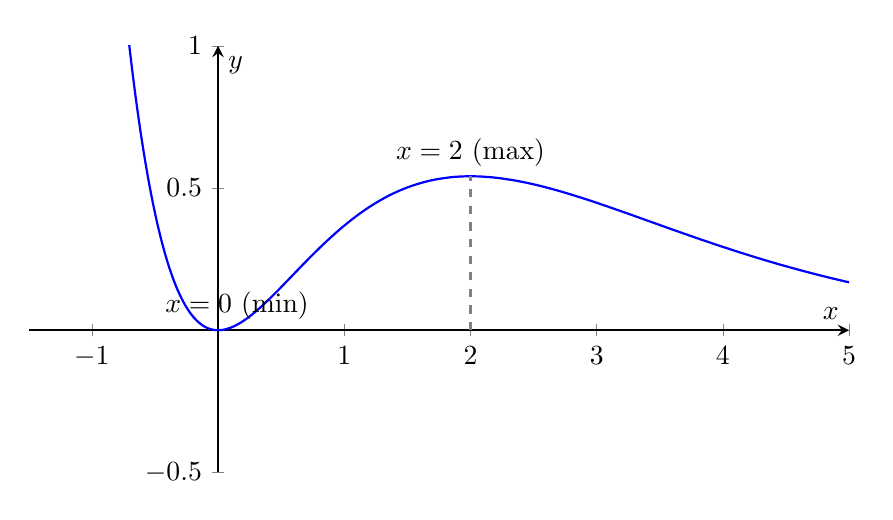
\begin{tikzpicture}[scale=1.0]
\begin{axis}[
  width=12cm,height=7cm,
  axis lines=middle,
  xlabel={$x$},ylabel={$y$},
  xmin=-1.5,xmax=5,
  ymin=-0.5,ymax=1,
  samples=200,domain=-1.5:5,
  smooth,thick
]
\addplot[blue] {x^2*exp(-x)};
\addplot[dashed,gray] coordinates {(0,0) (0,0)};
\addplot[dashed,gray] coordinates {(2,0) (2,{4*exp(-2)})};
\node[above left] at (axis cs:0.8,0) {$x=0$ (min)};
\node[above] at (axis cs:2,{4*exp(-2)}) {$x=2$ (max)};
\end{axis}
\end{tikzpicture}
\end{center}
\begin{example}
$f(x)=|x|$ функцийн график “V” хэлбэртэй байдаг. 

\[
f(x)=
\begin{cases}
 -x, & x<0,\\[3pt]
  x, & x\ge 0.
\end{cases}
\]
тул уламжлал нь
\[
f'(x)=
\begin{cases}
 -1, & x<0,\\[3pt]
 +1, & x>0.
\end{cases}
\]
$x=0$ дээр $f'(x)$ оршихгүй ($\lim_{x\to0^-}f'(x)=-1$, $\lim_{x\to0^+}f'(x)=1$), учир $x=0$ — сэжигтэй цэг болно.

\textbf{Өсөлт–бууралтын шинжилгээ:}
\begin{itemize}
  \item $x<0$ үед $f'(x)=-1<0$ → $f$ \textbf{буурах}.
  \item $x>0$ үед $f'(x)=+1>0$ → $f$ \textbf{өсөх}.
\end{itemize}

Тиймээс $f(x)$ нь $x=0$ цэгт буурахаас өсөхөд шилжиж байна.
Иймд $x=0$ нь \textbf{локал минимум} ба $f(0)=0$.
\begin{center}
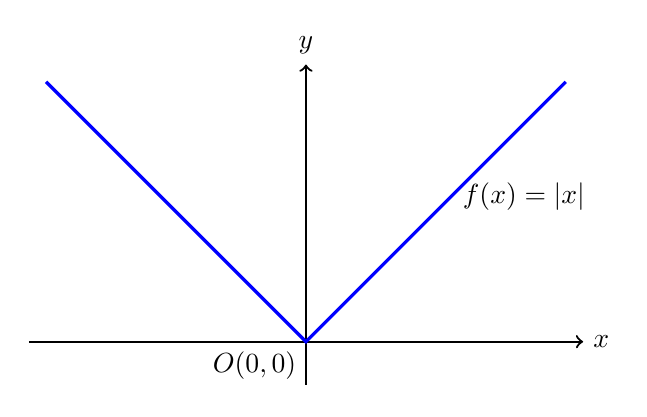
\begin{tikzpicture}[scale=1.1]

% --- координатын тэнхлэг ---
\draw[->, thick] (-3.2,0) -- (3.2,0) node[right] {$x$};
\draw[->, thick] (0,-0.5) -- (0,3.2) node[above] {$y$};

% --- |x| функцийн график ---
\draw[blue, very thick] (-3,3) -- (0,0) -- (3,3);

% цэгийн тэмдэглэгээ
\node[below left] at (0,0) {$O(0,0)$};
\node[above right] at (1.7,1.4) {$f(x)=|x|$};


\end{tikzpicture}
\end{center}
Графикаас $x=0$ — локал болон глобаль минимум байна.
\end{example}

Энэ аргаар функцийн өсөлт–бууралтын завсар, түүгээр дамжуулан локал экстремумыг тодорхойлох аргийг \emph{1-р уламжлалын тэмдэгийн тест} гэж нэрлэдэг.
\subsection{Экстермум олох}
$y=f(x)$ функцийн $[a,b]$ завсар дээрх локал экстермум олохын тулд дараах алхамуудыг гүйцэтгэх шаардлагатай.
\begin{enumerate}
  \item $f'(x)$ уламжлалыг олж түүний уламжлал оршихгүй цэгүүд болон $f'(x)=0$ тэгшитгэл бодож сэжигтэй цэгүүдийг олно. 
  \item \textit{I уламжлалын тестээр (тэмдэгийн хүснэгт):} Сэжигтэй цэг $c$-г дайрч гарахдаа $f'$-ийн тэмдэг өөрчлөгдөх байдлыг шалган локал максимум, локал минимум эсвэл экстермум биш эсэхийг тодорхойлоно. Хэрэв  $f'$-ийн тэмдэг $+\to -$ бол максимум, $-\to +$ бол минимум, тэмдэг өөрчлөгдөхгүй бол экстремум биш байна.
\end{enumerate}  
\begin{example}
$f(x)=\dfrac{x+1}{x^2+1}$ \quad (муж $x\in\mathbb{R}$).
\[
f'(x)=\frac{(1)(x^2+1)-(x+1)(2x)}{(x^2+1)^2}
=\frac{x^2+1-2x(x+1)}{(x^2+1)^2}
=\frac{-x^2-2x+1}{(x^2+1)^2}.
\]
Сэжигтэй цэгүүд: $-x^2-2x+1=0 \;\Rightarrow\; x=\frac{-2\pm\sqrt{4+4}}{2}=-1\pm\sqrt{2}$.
Иймд $x=-1-\sqrt2$-д $f'$ тэмдэг $+\to -$ (максимум), $x=-1+\sqrt2$-д $-\to +$ (минимум) болно.
\[
f(-1-\sqrt2)=\frac{-\sqrt2}{( (-1-\sqrt2)^2+1)} \quad\text{ба}\quad
f(-1+\sqrt2)=\frac{\sqrt2}{( (-1+\sqrt2)^2+1)}.
\]
Дүгнэлт: $x=-1-\sqrt2$ дээр локал максимум, $x=-1+\sqrt2$ дээр локал минимум.
\end{example}

$y=f(x)$ функцийн $[a,b]$ завсар дээрх глобал экстермум олохын тулд дараах алхамуудыг гүйцэтгэх шаардлагатай.
\begin{enumerate}
  \item Локал экстермумийн цэгүүдийг олж локал экстремумын цэгүүд дээрх функцийн утгууд $f(c)$-г бодно.
  \item Төгсгөлүүдийн цэгүүд дээрх утгууд $f(a), f(b)$-г бодож экстремумын цэгүүд дээрх функцийн утгуудтай харьцуулан эдгээрээс глобал экстермум утгаа тодорхойлно.
  \end{enumerate}  
\begin{example}
$f(x)=x^3-3x$-ийн глобал экстремумыг $[-2,2]$ дээр ол.
\[
f'(x)=3x^2-3=3(x^2-1)=0 \;\Rightarrow\; x=\pm1.
\]
Төгсгөлийн цэгүүд: $x=-2,\,2$. Утгууд:
\[
f(-2)=-8+6=-2,\quad f(-1)=-1+3=2,\quad f(1)=1-3=-2,\quad f(2)=8-6=2.
\]\\
\textbf{Дүгнэлт:} Хамгийн их утга $2$ нь $x=-1$ ба $x=2$ дээр; хамгийн бага утга $-2$ нь $x=-2$ ба $x=1$ дээр.    
\end{example}
\begin{example}
$f(x)=x\,e^{-x^2}$-ийн глобал экстремумыг $\mathbb{R}$ дээр ол.
\[
f'(x)=e^{-x^2}(1-2x^2)=0 \;\Rightarrow\; x=\pm \frac{1}{\sqrt2}.
\]
Утгууд:
\[
f\!\left(\tfrac{1}{\sqrt2}\right)=\frac{1}{\sqrt2}\,e^{-1/2}=\frac{1}{\sqrt{2e}},\qquad
f\!\left(-\tfrac{1}{\sqrt2}\right)=-\frac{1}{\sqrt{2e}}.
\]
Мөн $\lim_{x\to\pm\infty}f(x)=0$. \\
\textbf{Дүгнэлт:} Хамгийн их утга $f_{\max}=\dfrac{1}{\sqrt{2e}}$ нь $x=\dfrac{1}{\sqrt2}$ дээр;хамгийн бага утга $f_{\min}=-\dfrac{1}{\sqrt{2e}}$ нь $x=-\dfrac{1}{\sqrt2}$ дээр.
\end{example}
\begin{example}
$f(x)=|x|+(x-1)^2$-ийн абсолют экстремумыг $\mathbb{R}$ дээр ол.

Модулийг задлахын тулд хоёр мужид хуваая. 
\[
\begin{cases}
x\ge 0:\; f(x)=x+(x-1)^2 = x^2+(-1)x+1, \quad f'(x)=2x-1,\\[2pt]
x<0:\; f(x)=-x+(x-1)^2 = x^2-3x+1, \quad f'(x)=2x-3.
\end{cases}
\]
Сэжигтэй цэгүүд:
\[
x> 0:\; 2x-1=0 \Rightarrow x=\tfrac12\ (\text{тэгээс их тул шийд болно}),\qquad
x<0:\; 2x-3=0 \Rightarrow x=\tfrac32\ \text{(энэ нь тэгээс бага биш тул шийд биш)}.
\]
Мөн $x=0$ дээр $|x|$-ийн уламжлал тасардаг тул сэжигтэй цэг болох тул \emph{заавал} шалгана.
Утгууд:
\[
f\!\left(\tfrac12\right)=\tfrac12+\Big(\tfrac12-1\Big)^2=\tfrac12+\tfrac14=\tfrac34,\qquad
f(0)=0+1=1.
\]
$x\to\pm\infty$ үед $f(x)\sim x^2\to\infty$. \\
\textbf{Дүгнэлт:} Хамгийн бага утга $f_{\min}=\dfrac{3}{4}$ нь $x=\dfrac12$ дээр, хамгийн их утга байхгүй (∞ руу өснө)    
\end{example} 
\subsection{Лопиталын дүрэм}

\begin{theorem}[Лопитал]
$f,g$ нь $a$ цэгийн орчинд дифференциалчлагддаг, $g'(x)\ne0$, мөн $x\to a$ үед $f$ ба $g$ нь $0$ (эсвэл $\pm\infty$) руу ойртдог байг. Хэрэв
\[
\lim_{x\to a}\frac{f'(x)}{g'(x)}=L \text{ оршвол}\quad 
\lim_{x\to a}\frac{f(x)}{g(x)}=L.
\]
\end{theorem}

\begin{prof}
Кошийн теоремыг $[x,a]$ дээр хэрэглэн $\dfrac{f'(c)}{g'(c)}=\dfrac{f(x)-f(a)}{g(x)-g(a)}$ ($f(a)=g(a)=0$) авна. $x\to a$ үед $c\to a$.
\end{prof}
\begin{example}
\begin{multicols}{2}
\begin{enumerate}[itemsep=2pt]
\item $\displaystyle \lim_{x\to0}\frac{\sin x}{x}=\lim\frac{\cos x}{1}=1.$
\item $\displaystyle \lim_{x\to\infty}\frac{\ln x}{x}=\lim\frac{1/x}{1}=0.$
\item $\displaystyle \lim_{x\to0}\frac{e^x-1}{x}=\lim\frac{e^x}{1}=1.$
\item $\displaystyle \lim_{x\to0}\frac{1-\cos x}{x^2}=\lim\frac{\sin x}{2x}=\frac12.$
\end{enumerate}
\end{multicols}
    
\end{example}
% ===============================================================
\section*{Семинар}

\begin{enumerate}
  \item Дифференциал ашиглан ойролцоогоор бод
  \begin{enumerate}
  \item  \(\sin(0.12)\). (Радианаар авч үзнэ.)
  \item \((1.02)^5\)
\end{enumerate}
  \item Шүргэгч ба нормаль шулууны тэгшитгэлийг ол.    
  \begin{enumerate}
      \item \(y=\sin x+\cos x\)-ийн \(x=\tfrac{\pi}{3}\) цэг дээрх 
  \item \(y=x^2-3x+2\)-ийн \(x=1\) цэг дээрх 
  \item  \(x=\cos t,\; y=\sin t\) \(t=\tfrac{\pi}{4}\) дээрх
  \end{enumerate}
    \item $y=\sqrt{2x-x^2}$ функц $(0;1)$  дээр өсдөг, $(1;2)$ дээр буурдаг болохыг харуул.
    \item $y=x^3+x$ өсдөг болохыг батал.
    \item Өсөх, буурах завсарыг ол.
    \begin{enumerate}
        \item $y=(x-2)^5(2x+1)^4$
        \item $y=x-e^x$
        \item $y=\dfrac{1-x+x^2}{1+x+x^2}$
        \item $y=xe^{-x}$
        \item $y=\dfrac{1}{\ln x}$
        \item $y=x^2-\ln x$
        \item $y=x-\sin 2x,\quad (0<x<\pi)$
        \item $y=x+\cos x$
    \end{enumerate}
    \item Локал экстермум ол.
    \begin{enumerate}
        \item $y=2x^3-3x^2$
        \item $y=2x^3-6x^2+18x-1$
        \item $y=x^2\cdot \sqrt{x^2+2}$
        \item $y=x-\ln (x+1)$
        \item $y=\sin x$
        \item $y=x\sin x+\cos x-\dfrac{x^2}{4}, \quad -\dfrac{\pi}{2}\leq x\leq \dfrac{\pi}{2}$
        \item $y=\dfrac{1+3x}{\sqrt{4+5x^2}}$
        \item $y=x-\ln(1+x^2)$
        \item $y=\sqrt[3]{(x^2-4)^2}$
        \item $y=2e^{3x}+3e^{-3x}$
    \end{enumerate}
    \item Глобал экстермум ол.
    \begin{enumerate}
        \item $y=x^4-2x^2+5, \quad [-2;2]$
        \item $y=x+2\sqrt{x} \quad [0;4]$
        \item $y=x^5-5x^4+5x^3+2,\quad [-1;1]$
        \item $y=\sqrt{100-x^2}, \quad [-6;8]$
        \item $y=\dfrac{1-x+x^2}{1+x+x^2}, \quad [0;1]$
        \item $y=x\sin x+\cos x-\dfrac{x^2}{4}, \quad -\dfrac{\pi}{2}\leq x\leq \dfrac{\pi}{2}$
        \item $y=\dfrac{1+3x}{\sqrt{4+5x^2}}, \quad [0;1]$
        \item $y=x-\ln(1+x^2)$
        \item $y=\sqrt[3]{(x^2-4)^2}, \quad [0;3]$
        \item $y=2e^{3x}+3e^{-3x}$
    \end{enumerate}
\end{enumerate}
\section*{Гэрийн даалгавар}
\begin{enumerate}
  \item Функцийн локал экстремумыг ол.
  \begin{enumerate}
  \item  $y = x^3 - 6x^2 + 9x - 4$ 
  \item $y = 2x^3 - x^4$ 
  \item $y = x(x-1)^3(x-2)^3$ 
  \item $y = x + \dfrac{1}{x}$ 
  \item $y = \dfrac{2x}{1+x^2}$ 
  \item $y = \dfrac{x^3 - 3x + 2}{x^3 + 2x + 1}$ 
  \item $y = \sqrt{2x - x^3}$ 
  \item $y = x^3\sqrt[3]{x - 1}$ 
  \item $y = x e^{-x}$
  \item $y = \sqrt{x}\,\ln x$ 
  \item $y = \dfrac{(\ln x)^2}{x}$
  \item $y = \cos x + \dfrac{1}{2}\cos 2x$ 
  \item $y = \dfrac{10}{1 + \sin^2 x}$ 
  \item $y = \arctan x - \dfrac{1}{2}\ln(1 + x^2)$ 
  \item $y = e^x \sin x$ 
  \item $y = |x|\, e^{-|x-1|}$
  \end{enumerate}
\item Өгөгдсөн завсар дээрх хамгийн их ба хамгийн бага утгыг ол.
  \begin{enumerate}
  \item  $f(x) = 2x$, $[-1; 5]$ 
  \item $f(x) = x^2 - 4x + 6$, $[-3; 10]$ 
  \item $f(x) = |x^2 - 3x + 2|$, $[-10; 10]$ 
  \item $f(x) = x + \dfrac{1}{x}$, $[0.01; 100]$ 
  \item $f(x) = \sqrt{5 - 4x}$, $[-1; 1]$ 
  \end{enumerate}
\item Дараах тэнцэтгэл бишүүдийг функцийн хамгийн их ба бага утга олох замаар батла.
   \begin{enumerate}
   \item $|3x - x^3| \le 2$, хэрэв $|x| \le 2$
   \item $\dfrac{1}{2^{p-1}} \le x^p + (1-x)^p \le 1$, хэрэв $0 \le x \le 1$ ба $p>1$.
  \item $x^m (a-x)^n \le 
    \dfrac{m^m n^n}{(m+n)^{m+n}}\, a^{m+n}$, хэрэв $m>0$, $n>0$, $0\le x\le a$.
  \item $\dfrac{x+a}{2^{(n-1)/n}} \le \sqrt[n]{x^n+a^n} \le x+a$, хэрэв $x>0,\, a>0,\, n>1$.
  \item $|a\sin x + b\cos x| \le \sqrt{a^2+b^2}$.
  \item $\dfrac{2}{3} \le \dfrac{x^2+1}{x^3+x+1} \le 2$, бүх $x \in \mathbb{R}$-д.
   \end{enumerate}
\item $y=ax^2+bx+c$ параболын $x=p, x=q$ цэгүүд дээрх шүргэгч шулуунууд $x=\dfrac{p+q}{2}$ цэг дээр огтолцохыг батал.
\item $y=x^2$ параболын $x=p, x=q$ цэгүүд дээрх шүргэгч шулуунууд перпиндикуляр бол огтолцолын цэг нь $y=-\dfrac{1}{4}$ шулуун дээр оршихыг батал.
\item $y=\dfrac{1}{x}$ функцийн $x=p ,\quad (p>0)$ цэг дээрх шүргэгч шулуун ба $ox$, $oy$ тэнхлэгүүдээр үүсэх гурвалжны талбай $p$-с хамаарахгүй тогтмол байхыг батал.
\end{enumerate}
